\chapter{Experimental results}
\label{ch:chapter_4}%

We introduced the Key Management Entity in the previous chapters and described its implementation details. Here, we will show three use cases to demonstrate that our implementation of the KME works as expected.

In all the following experiments, we will not use the Quantum Channel Simulator described in \ref{kme:qcs} and exploited during the development process. Instead, the KMEs will receive blocks from the Quantum Channel maintained in Politecnico di Milano. The goal is to provide examples of operations of the KME in situations that are as close to actual use case scenarios as possible. The details about how to boot and configure the quantum channel are out of the scope of this document.

All the experiments require the boot of the quantum channel and two cooperating KMEs, which are two KMEs linked to the different endpoints of the same quantum channel. We will refer to these KMEs as Alice and Bob to distinguish them.

We boot one KME with ID "Alice" on our machine. It listens to new blocks from the Quantum Channel on TCP port 9998 and listens to requests from the API on TCP port 5000. These settings must be defined before booting the KME, modifying its configuration file. When  everything is ready, it is possible to start Alice with the command:

\begin{minted}{bash}
poetry run python -m kme
\end{minted}

Then, we boot another KME with ID "Bob" on the same machine. So, Alice and Bob are both executing on localhost. Bob listens to new blocks from the Quantum Channel on TCP port 9999 and listens to requests from the API on TCP port 3000. Now, it is possible to start Bob with the command above.

There should not be an overlap between TCP ports because Alice and Bob are running on the same machine, so this would lead to undesired network conflicts.

Alice and Bob receive blocks from the quantum channel and store them locally during the execution. Chapter 2 deepened the details of the cooperation between the two KMEs and their communication with the quantum channel.

In the following figures, Alice and Bob have been booted and are receiving the very same blocks from the quantum channel.

\begin{figure}[H]
    \centering
    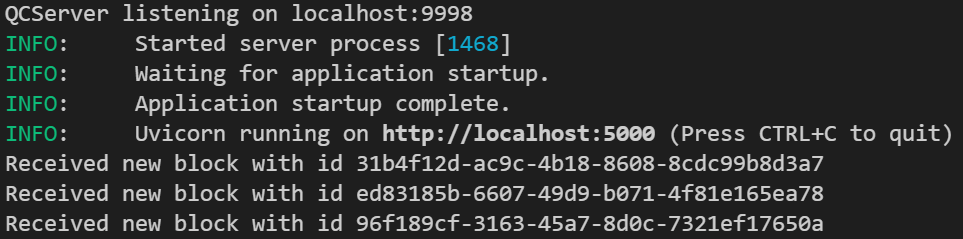
\includegraphics[width=0.8\textwidth]{Images/alice.png}
    \caption{Alice listening on TCP port 5000.}
    \label{fig:alice}
\end{figure}

\begin{figure}[H]
    \centering
    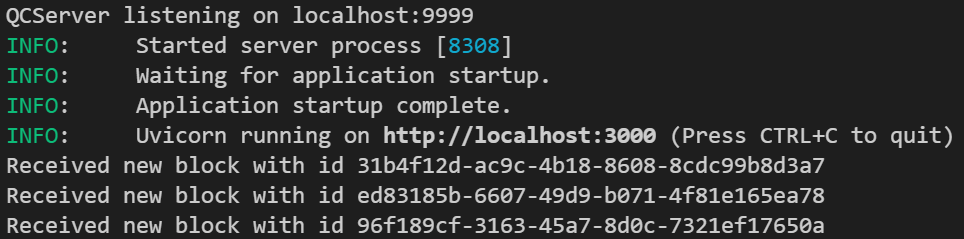
\includegraphics[width=0.8\textwidth]{Images/bob.png}
    \caption{Bob listening on TCP port 3000.}
    \label{fig:bob}
\end{figure}

\section{First experiment: successful generation of a new key}
We want to exhibit regular communication between Alice and Bob in this first experiment. In particular, we request to Alice the generation of one key of length 256 bits. Alice responds with a key containing material of length 256 and a UUID.
Then, we request Bob to retrieve the key associated with the given UUID. If Bob responds with the very same key produced by Alice, then the experiment is successful.

Let us start the experiment. We request the generation of a new key of length 256 to Alice. The following is our HTTP request:

\begin{minted}{bash}
http://localhost:5000/api/v1/keys/BobApp/enc_keys?number=1&size=256
\end{minted}

Alice answers with an HTTP response having the following Key Container object as body:

\begin{minted}{json}
{
  "keys": [{
      "key_ID": "5df98759-6705-4de6-8f76-9c37adba7d82",
      "key": "/otfMnKVYI57Km2IA2Bs1jZAi5e9bBtli/7j5Vn1MQw="
    }]
}
\end{minted}

Now, we send Bob an HTTP GET request containing the above key\_ID, that is, the UUID of the key generated by Alice. Here is our HTTP request to Bob:

\begin{minted}{bash}
http://localhost:3000/api/v1/keys/AliceApp/
dec_keys?key_ID=5df98759-6705-4de6-8f76-9c37adba7d82
\end{minted}

The following is Bob's answer, with HTTP status code 200:
\begin{minted}{json}
{ "keys": [{
      "key_ID": "5df98759-6705-4de6-8f76-9c37adba7d82",
      "key": "/otfMnKVYI57Km2IA2Bs1jZAi5e9bBtli/7j5Vn1MQw="
    }]
}
\end{minted}

Bob returns the same key produced by Alice, confirming a successful communication between them.

\section{Second experiment: failure retrieving a key without the needed blocks}
In this second experiment, we focus on the communication between Alice and Bob again. Now, however, we analyze a situation where an error occurs. In particular, after Alice gives us one key with a material of length 256, we manually delete all the local database entries where Bob stores the blocks received from the Quantum Channel. When we ask Bob to retrieve the key associated with the given UUID, it cannot re-build that key. In fact, after reading from the shared database the instructions about how to re-build the key, Bob does not find the necessary blocks in its local database of blocks. This situation forces Bob to respond to our retrieval request with an error message.

Let us start the experiment. We request the generation of a new key of length 256 to Alice. The following is our HTTP request:

\begin{minted}{bash}
http://localhost:5000/api/v1/keys/BobApp/enc_keys?number=1&size=256
\end{minted}

Alice answers with an HTTP response having the following Key Container object as body:

\begin{minted}{json}
{ "keys": [{
      "key_ID": "4610bc87-271a-4fd2-a01c-4c8fc5498ed5",
      "key": "2WCmDSuiE1g7heV2rlhSgt2qflgC/NGUqmJcAM5FiD0="
    }]
}
\end{minted}

Now, we manually delete all the blocks from Bob's local DB. Asking for the key produced by Alice, we expect to get an HTTP error response. Here is our HTTP request to Bob:

\begin{minted}{bash}
http://localhost:3000/api/v1/keys/AliceApp/
dec_keys?key_ID=4610bc87-271a-4fd2-a01c-4c8fc5498ed5
\end{minted}

The following is Bob's answer, with HTTP status code 400:

\begin{minted}{json}
{ "message": "One or more keys specified are not found on KME" }
\end{minted}

The message that the KME returns to the calling SAE is generic and points out that it could not re-build the requested key. In Bob's logging console, we can also find the following message:

\begin{minted}{bash}
ERROR: Block with UUID c3c8a268-9a26-41d4-ae77-105b0dd360fb not found
\end{minted}

This message confirms that the error was produced by the inability of KME Bob to retrieve a block pointed out in the instructions for re-building the key with the given UUID. So, our experiment has been successful.

\label{ch4:exp3}
\section{Third experiment: successful cooperation between three KMEs}
We consider a more sophisticated situation in the third experiment than previously described. Up to now, we have focused on two cooperating KMEs linked to the same quantum channel. Each KME received blocks from the same quantum channel. However, our implementation of a KME can handle blocks coming from multiple quantum channels. Each quantum channel is identified by a UUID, which is embedded into the block when sent to the KME. Therefore, the fields of a block sent to the KME are:

\begin{itemize}
 	\item \textit{block\_id}: the UUID of the block;
	\item \textit{material}: the block material;
	\item \textit{timestamp}: the timestamp of the block;
	\item \textit{link\_id}: the UUID of the quantum channel that produced this block.
\end{itemize}

One master SAE wants to request the generation of keys produced from blocks of a particular quantum channel. In order to do so, it has to exploit the HTTP POST request \textit{enc\_keys}, specifying "link\_id" as an "extension mandatory" parameter. For more details about the structure of this API interface, please see \ref{kme:key_gen}.

By now, we manually provide the UUID of the quantum channel. In the last chapter of this document, we will see one future development purpose for automating the process.

So, in this experiment, we will consider two quantum channels:
\begin{itemize}
    \item QC\_A, associated with the UUID de2e6bbe-4897-40df-8532-b7425a6f57d9;
    \item QC\_B, associated with the UUID 231656cb-d062-4897-bb11-8d3a551e720c.
\end{itemize}

Then, we will consider three KMEs:
\begin{itemize}
    \item Alice, which receives blocks from both QC\_A and QC\_B;
    \item Bob\_A, which receives blocks only from QC\_A;
    \item Bob\_B, which receives blocks only from QC\_B;
\end{itemize}

Therefore, Alice and Bob\_A cooperate through the QC\_A, while Alice and Bob\_B cooperate through the QC\_B. Bob\_A and Bob\_B do not cooperate.

Alice and Bob\_A will use the same port as in the previous experiment. Bob\_B, instead, will listen for new blocks coming from QC\_B on TCP port 9997 and listen to API requests on TCP port 8000.

\begin{figure}[H]
    \centering
    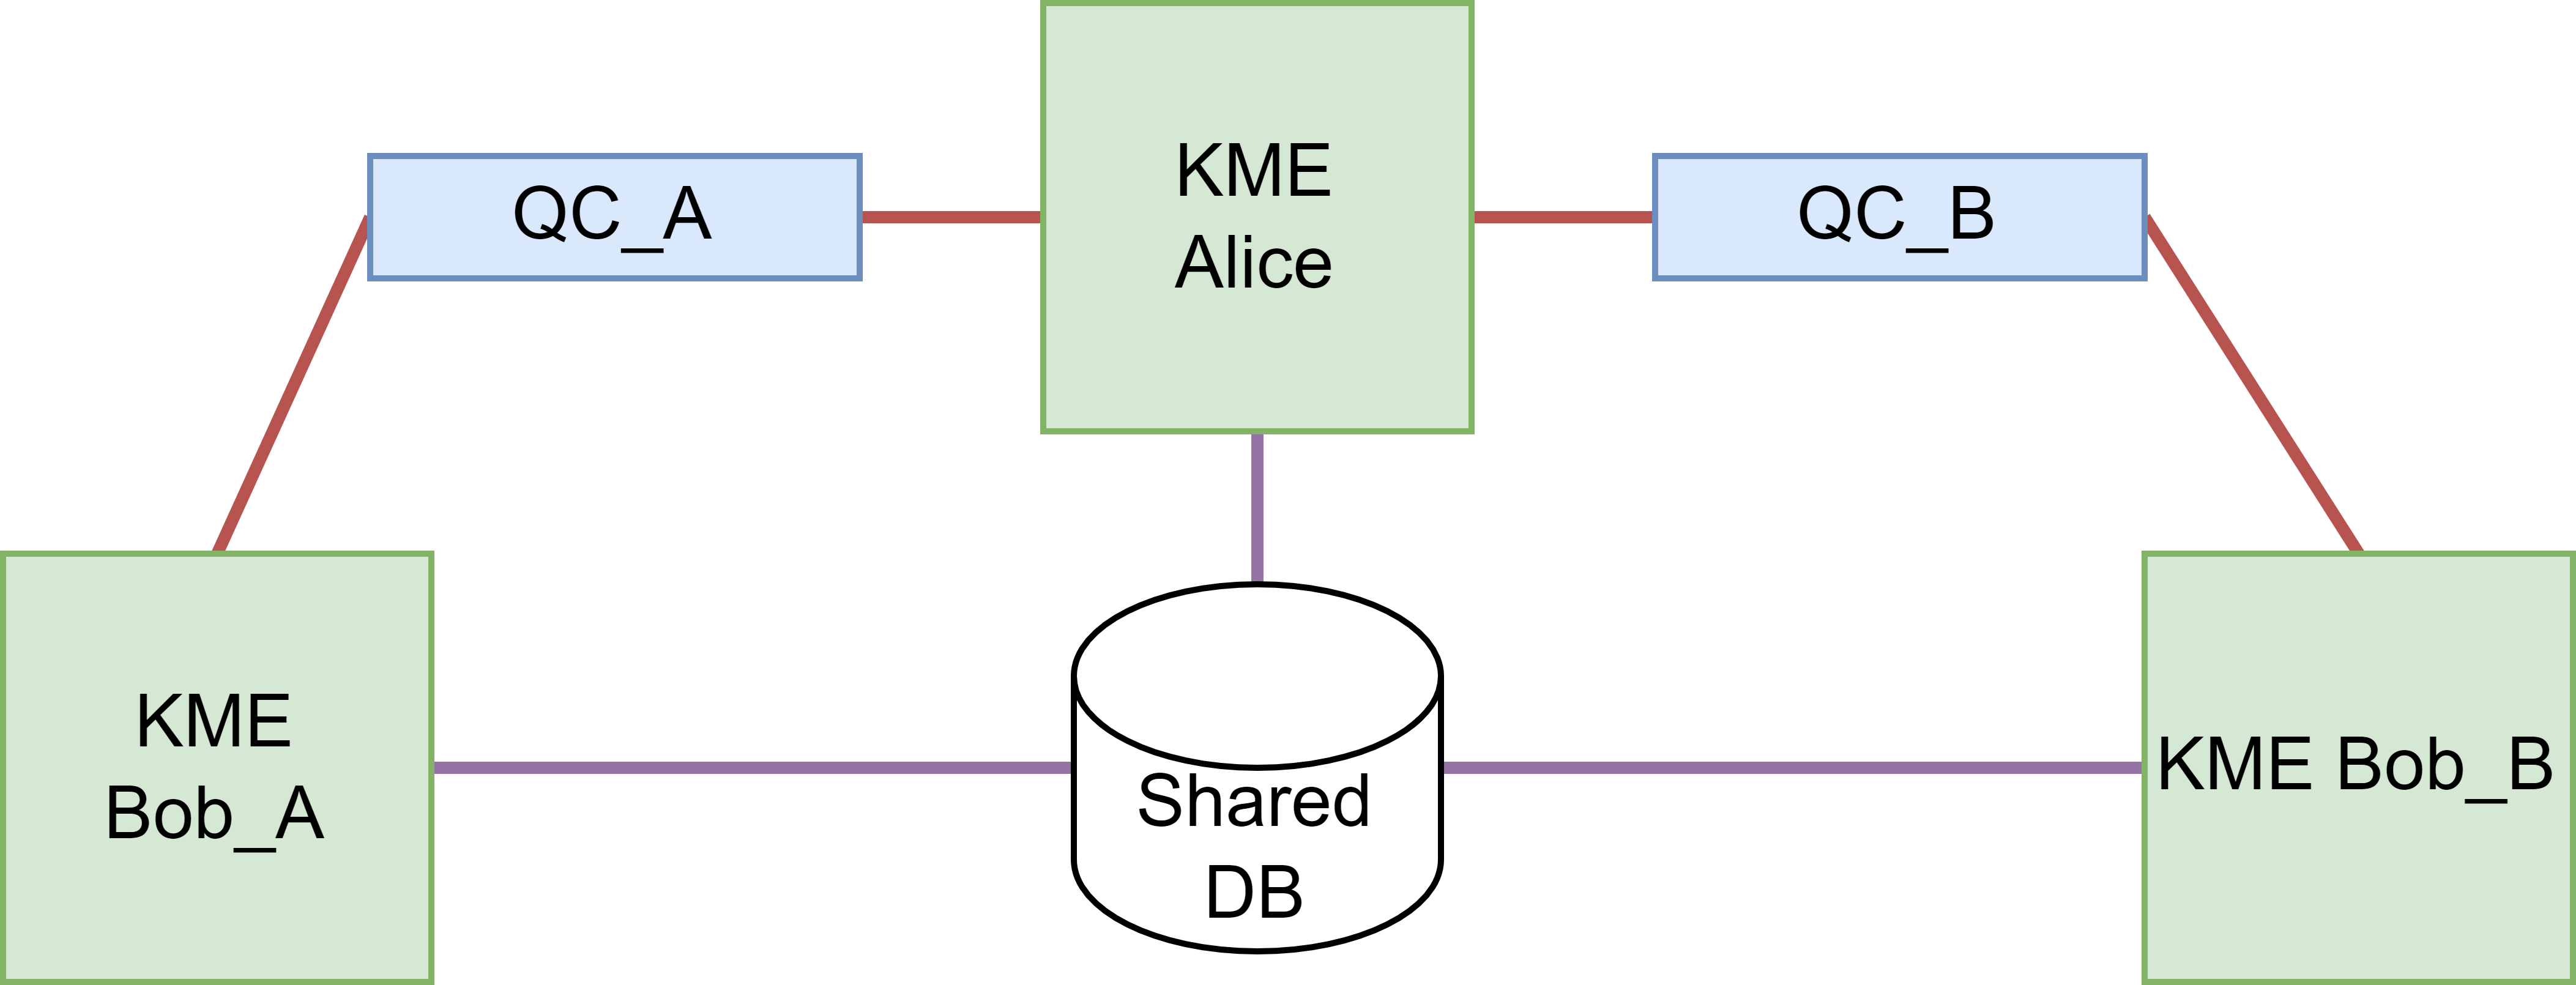
\includegraphics[width=1.0\textwidth]{Images/Third experiment.png}
    \caption{The topology of the third experiment.}
    \label{fig:third_exp}
\end{figure}

In this experiment, we will request Alice to generate a new key of length 256 bits exploiting blocks coming from the QC\_A. Then, we will request Bob\_A to retrieve the new key. Bob\_A cooperates with Alice through the QC\_A, so we expect to receive a successful HTTP response. Then, we will request Bob\_B to retrieve the very same key. However, Bob\_B does not cooperate with Alice through QC\_A, so we expect to receive an HTTP error response. Indeed, Bob\_B does not receive blocks from QC\_A, so it cannot find the blocks listed in the instructions shared between all the KMEs through the shared DB.

Let the experiment begin.
First, we request Alice to generate a new key of length 256 bits manipulating blocks from QC\_A. In order to do so, we exploit the HTTP POST request method \textit{enc\_keys}. The following is the request URL of the HTTP request:

\begin{minted}{bash}
http://localhost:5000/api/v1/keys/Bob_A_App/enc_keys
\end{minted}

While the following is the body of the HTTP request:
\begin{minted}{json}
{
  "number": 1,
  "size": 256,
  "extension_mandatory": [
    {"link_id": "de2e6bbe-4897-40df-8532-b7425a6f57d9"}
  ]
}
\end{minted}

Alice uses the blocks produced by the quantum channel associated with the link\_id specified in the request body. Then, it sends us an HTTP response with status code 200 and the following body, which is a Key Container object with the newly generated key:
\begin{minted}{json}
{ "keys": [{
      "key_ID": "afe2b30e-206b-410c-ab51-63d2d7726a12",
      "key": "eVzqbEODx8fxkQVnGgEys4aztzat94nP96SCcYVZSHE="
    }]
}
\end{minted}

Now, we use the key\_ID of the newly-generated key for asking Bob\_A and Bob\_B to re-build that key.

The HTTP request we send to them is the same:

\begin{minted}{bash}
http://localhost:3000/api/v1/keys/AliceApp/
dec_keys?key_ID=afe2b30e-206b-410c-ab51-63d2d7726a12
\end{minted}

However, the HTTP responses are different, as we expected. The HTTP response of Bob\_A has status code 200, and its body contains the same key returned by Alice:
\begin{minted}{json}
{ "keys": [{
      "key_ID": "afe2b30e-206b-410c-ab51-63d2d7726a12",
      "key": "eVzqbEODx8fxkQVnGgEys4aztzat94nP96SCcYVZSHE="
    }]
}
\end{minted}

Bob\_B's HTTP response, instead, has status code 400, and it does not contain the key associated with the given UUID. We repeat that this behavior is the one desired. Bob\_B does not know the blocks generated by the QC\_A: only Alice and Bob\_A know them. The public instructions on how to re-build the key with UUID afe2b30e-206b-410c-ab51-63d2d7726a12 are not enough to know the key material associated with that UUID. The shared DB does not compromise the security assumptions of the system in any way.